\newpage
\section{Entwurf und Aufbau der Datensammlungsumgebung}
TBD

\subsection{Integration diverser Datenströme in einem einheitlichen Datenkorpus}
Die erste Datenquelle für die Datensammlungsumgebung ist die Anwendungsschnittstelle der Tagesschau. Diese ist eine Nachrichtensendung der Arbeitsgemeinschaft der öffentlich-rechtlichen Rundfunkanstalten der Bundesrepublik Deutschland (ARD) . Über diese Schnittstelle ist es möglich, Beiträge der Website www.tagesschau.de im JavaScript Object Notation (JSON) Format abzufragen. 
Die Schnittstelle ist mit einer OpenAPI Specification dokumentiert, über welche alle Informationen bezogen werden können. Der Zugriff auf diese Schnittstelle ist auf 60 Aufrufe pro Stunde limitiert. Darüber hinaus ist lediglich die nicht-kommerzielle Nutzung gestattet. Zudem dürfen gesammelte Inhalte, mit Ausnahme der unter der Creative Common (CC) Lizenz stehenden Inhalte, nicht weiter veröffentlicht werden. \footcite [Vgl.][]{Fischer.2024}

Die Schnittstelle gruppiert sich in 4 Themensegmente, welche über eigene Endpunkte verfügen. 
\begin{itemize}
    \item Homepage - Abfrage von Nachrichten und Eilmeldungen der Startseite
    \item News - Abfrage von sämtlichen Nachrichten und Eilmeldungen
    \item Channels - Abfrage von Kanälen
    \item Search - Allgemeine Suche über alle Inhalte der Plattform
\end{itemize}
Jeder Endpunkt ist gemäß dem Paradigma Representational State Transfer (REST) konstruiert und wird entsprechend über das Hypertext Transfer Protocol (HTTP) abgefragt. \footcite [Vgl.][]{Fischer.2024}

Für die erste Umsetzung der Datensammlungsumgebung ist es ausreichend, den News Endpunkt zu konsumieren. Dieser gibt eine Liste von News Objekten zurück, wie im \ref{Anhang} beschrieben. Diese enthält folgende Informationen:


\begin{table}   
    \centering
    \caption{Attribute Tageschau API Response}
    \label{tab:Attribute Tageschau API Response}
    \begin{tabular}{|c|p{11cm}|} \hline 
        news & Bildet das Hauptelement, welches die verschiedenen Nachrichten enthält \\ \hline 
        sophoraId & Eindeutige Identifikationsnummer \\ \hline 
        externalId & Zusätzliche eindeutige Identifikationsnummer \\ \hline 
        title & Titel der Nachricht \\ \hline 
        teaserImage & Enthält Informationen über das Vorschaubild der Nachricht \\ \hline 
        date & Das Veröffentlichungsdatum des Artikels \\ \hline 
        tracking & Liste von Objekten, welche Tracking-Informationen beinhalten\\ \hline 
        tags & Liste von Objekten, welche Schlagwörter enthalten \\ \hline 
        updateCheckUrl & Adresse zur Überprüfung von Aktualisierungen der Nachricht \\ \hline 
        regionId & Identifikationsnummer, welche den regionalen Bezug der Nachricht angibt \\ \hline 
        details & Adresse zum Abfragen des Artikels im JSON Format \\ \hline 
        detailsweb & Adresse zum Abfragen des Artikels im HTTP Format \\ \hline 
        shareURL & Adresse zum Artikel zum Teilen der Nachricht über soziale Medien \\ \hline 
        topline & Kurze Zusammenfassung der Nachricht \\ \hline 
        firstSentence & Erster Satz der Nachricht \\ \hline 
        geotags & Enthält eine Liste von Objekten, welche die geographischen Informationen des Artikels beinhalten \\ \hline 
        type & Typ der Nachrichtenseite, z.B. \textit{news page} \\ \hline 
        nextPage & Adresse auf die nächste Seite mit weiteren Nachrichten \\ \hline 
        comments & Adresse zur Kommentarsektion eines Artikels, sofern vorhanden \\ \hline 
        ressort & Themenfeld des Artikels, z.B. \textit{ausland} \\ \hline 
        breakingNews & Boolescher Wert, ob der Artikel als Eilmeldung veröffentlicht wurde \\ \hline
    \end{tabular}
\end{table}
\begin{table}
\centering
\caption{Tracking-Objekte in der Tagesschau API}
\label{tab:Tracking Tageschau API}
\begin{tabular}{|c|p{11cm}|} \hline 
    \textbf{Tracking-Attribut} & \textbf{Beschreibung} \\ \hline 
        sid & Session Id zum Nachverfolgen des Nutzerverhaltens \\ \hline 
        src & Quelle des Artikels, zeigt z.B. auf den Kanal, aus welchem der Artikel stammt \\ \hline 
        ctp & Art des Inhaltes als technischer Kenner \\ \hline 
        pdt & Datum der Veröffentlichung (englisch: Publish Date Time) \\ \hline 
        otp & Art des Inhaltes als fachlicher Kenner, z.B. \textit{meldung} \\ \hline 
        cid & Eindeutige Identifikationsnummer \\ \hline 
        pti & Titel der Seite (englisch: Page Title) \\ \hline 
        pcr & Flaggen Attribut, Verwendung ist unbekannt \\ \hline 
        type & Typ des Tracking Objektes, z.B. \textit{generic} \\ \hline
    \end{tabular}
\end{table}

Die erste Ebene der Datenstruktur enthält primär Metadaten zu einer Nachricht. Um den, für die Sammlung relevanten, Inhalt zu erhalten, sind die Referenzen auf die Details sowie die Kommentare aufzulösen. 
Dazu wird jeweils die Adresse aus dem jeweiligen Attribut aufgerufen. 

\newpage
Die Antwort für den Artikel erfolgt als JSON Objekt. Dieses enthält ebenfalls Metadaten, wie \textit{sophoraId}, \textit{externalId}, \textit{title} und \textit{date}, darüber hinaus aber auch den Artikel selbst. 
Der Inhalt ist in verschiedene Segmente aufgeteilt und entsprechend in der JSON-Antwort abgebildet. Der Inhalt eines Segments wird im \textit{value} Attribut gehalten, im \textit{type} Attribut wird bestimmt, um was es sich handelt (text, headline, box etc.).

Die Antwort für die Kommentarsektion erfolgt als HTML Seite. 
\begin{figure}
    \centering
    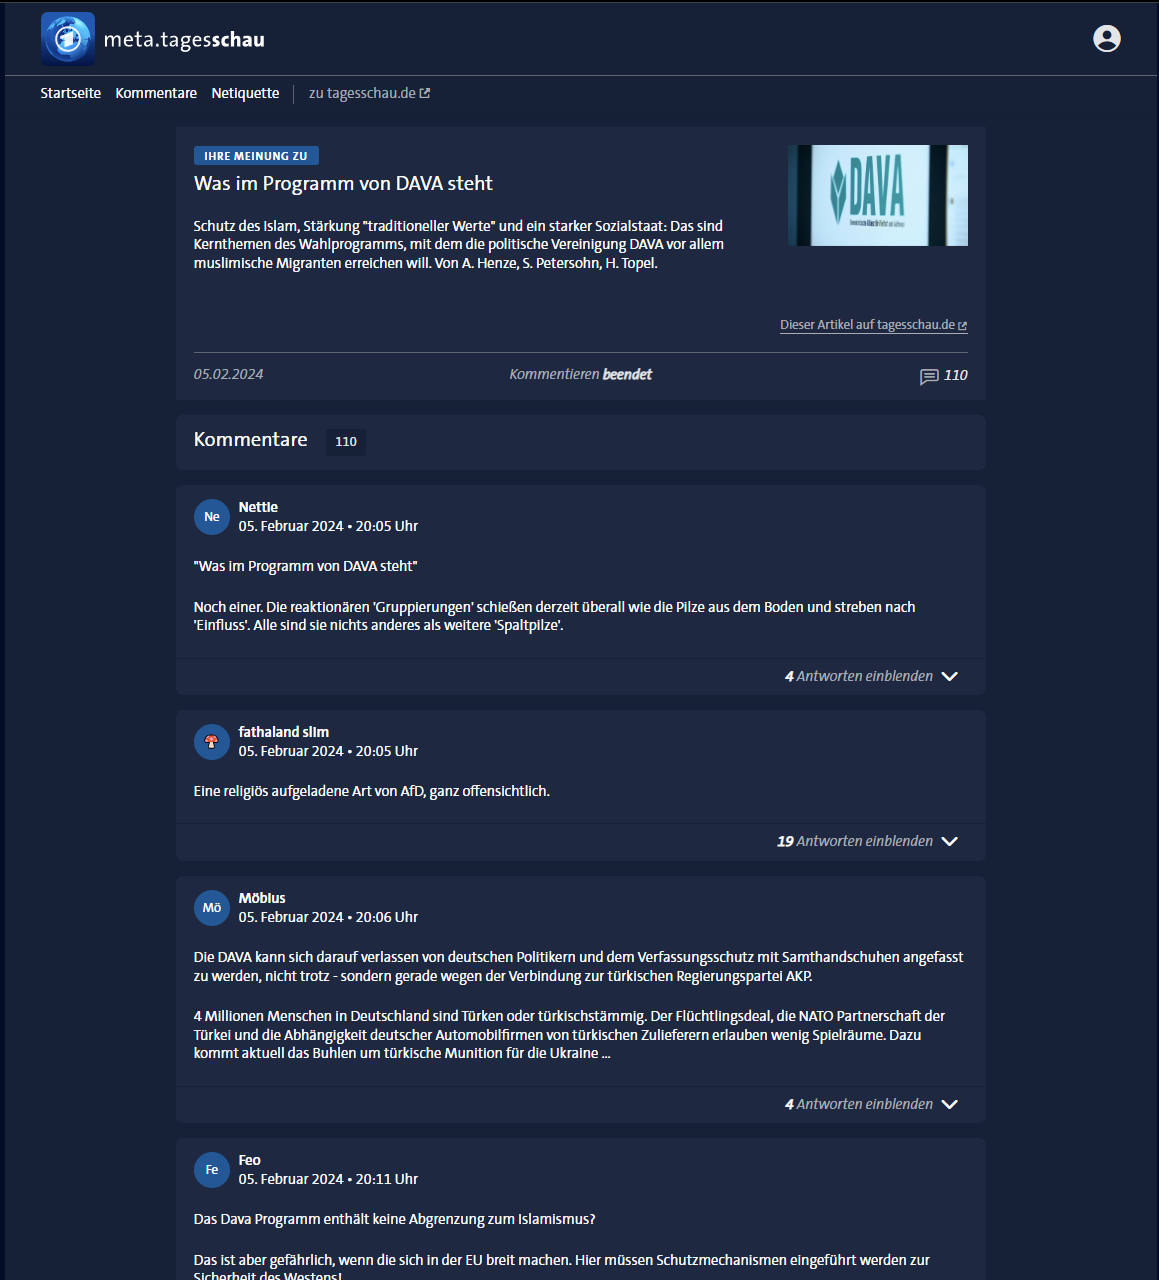
\includegraphics[width=1\linewidth]{abbildungen/Screenshot Comment Tagesschau.PNG}
    \caption{Tagesschau Kommentarsektion} 
    \label{fig:Tagesschau Kommentarsektion}
    Quelle: \fullcite{Norddeutscher_Rundfunk.2024}
\end{figure}

Aus Dieser lassen sich verschiedene Informationen beziehen.
\begin{itemize}
    \item Username
    \item Profilbild
    \item Datum und Uhrzeit des Kommentars
    \item Kommentar Text
    \item Anzahl der Antworten
    \item Anzahl der gesamten Kommentare zum Artikel
\end{itemize}

Die Kommentare werden in Seiten strukturiert und entsprechend nur teilweise zurückgegeben (engl. Paging). Dabei wird die Reihenfolge chronologisch bestimmt, beginnend mit den ersten Kommentaren. Das Konzept plant das Beziehen der ersten Seite der Kommentare.

\newpage

\begin{figure}
    \centering
    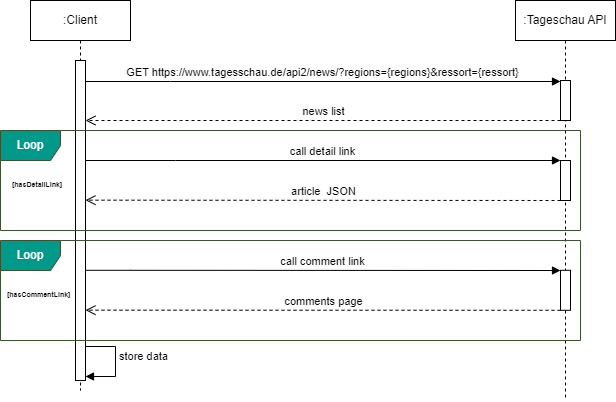
\includegraphics[width=1\linewidth]{abbildungen/Request Sequence.drawio.png}
    \caption{Abfragesequenz Datensammlung}
    \label{fig:Abfragesequenz Datensammlung}
\end{figure}
Der Ablauf der Datensammlung muss zwangsläufig mit dem initialen Abfragen der Tagesschau API starten, wie in der OpenAPI Spezifikation beschrieben. Anschließend können die Abfragen für den Artikeltext, sowie den Kommentaren stattfinden (siehe Abbildung \ref{fig:Abfragesequenz Datensammlung}). Um die Limitierung der Schnittstelle nicht zu überschreiten ist es notwendig, die zu machenden Aufrufe bestimmen zu können. Die Anzahl der benötigten Aufrufe lässt sich, auf Basis der geplanten Kommunikationsstruktur mit folgender Formel ausdrücken:

\(TotalRequests=1+(AmountArticles×2)\)

\newpage
\begin{figure}
    \centering
    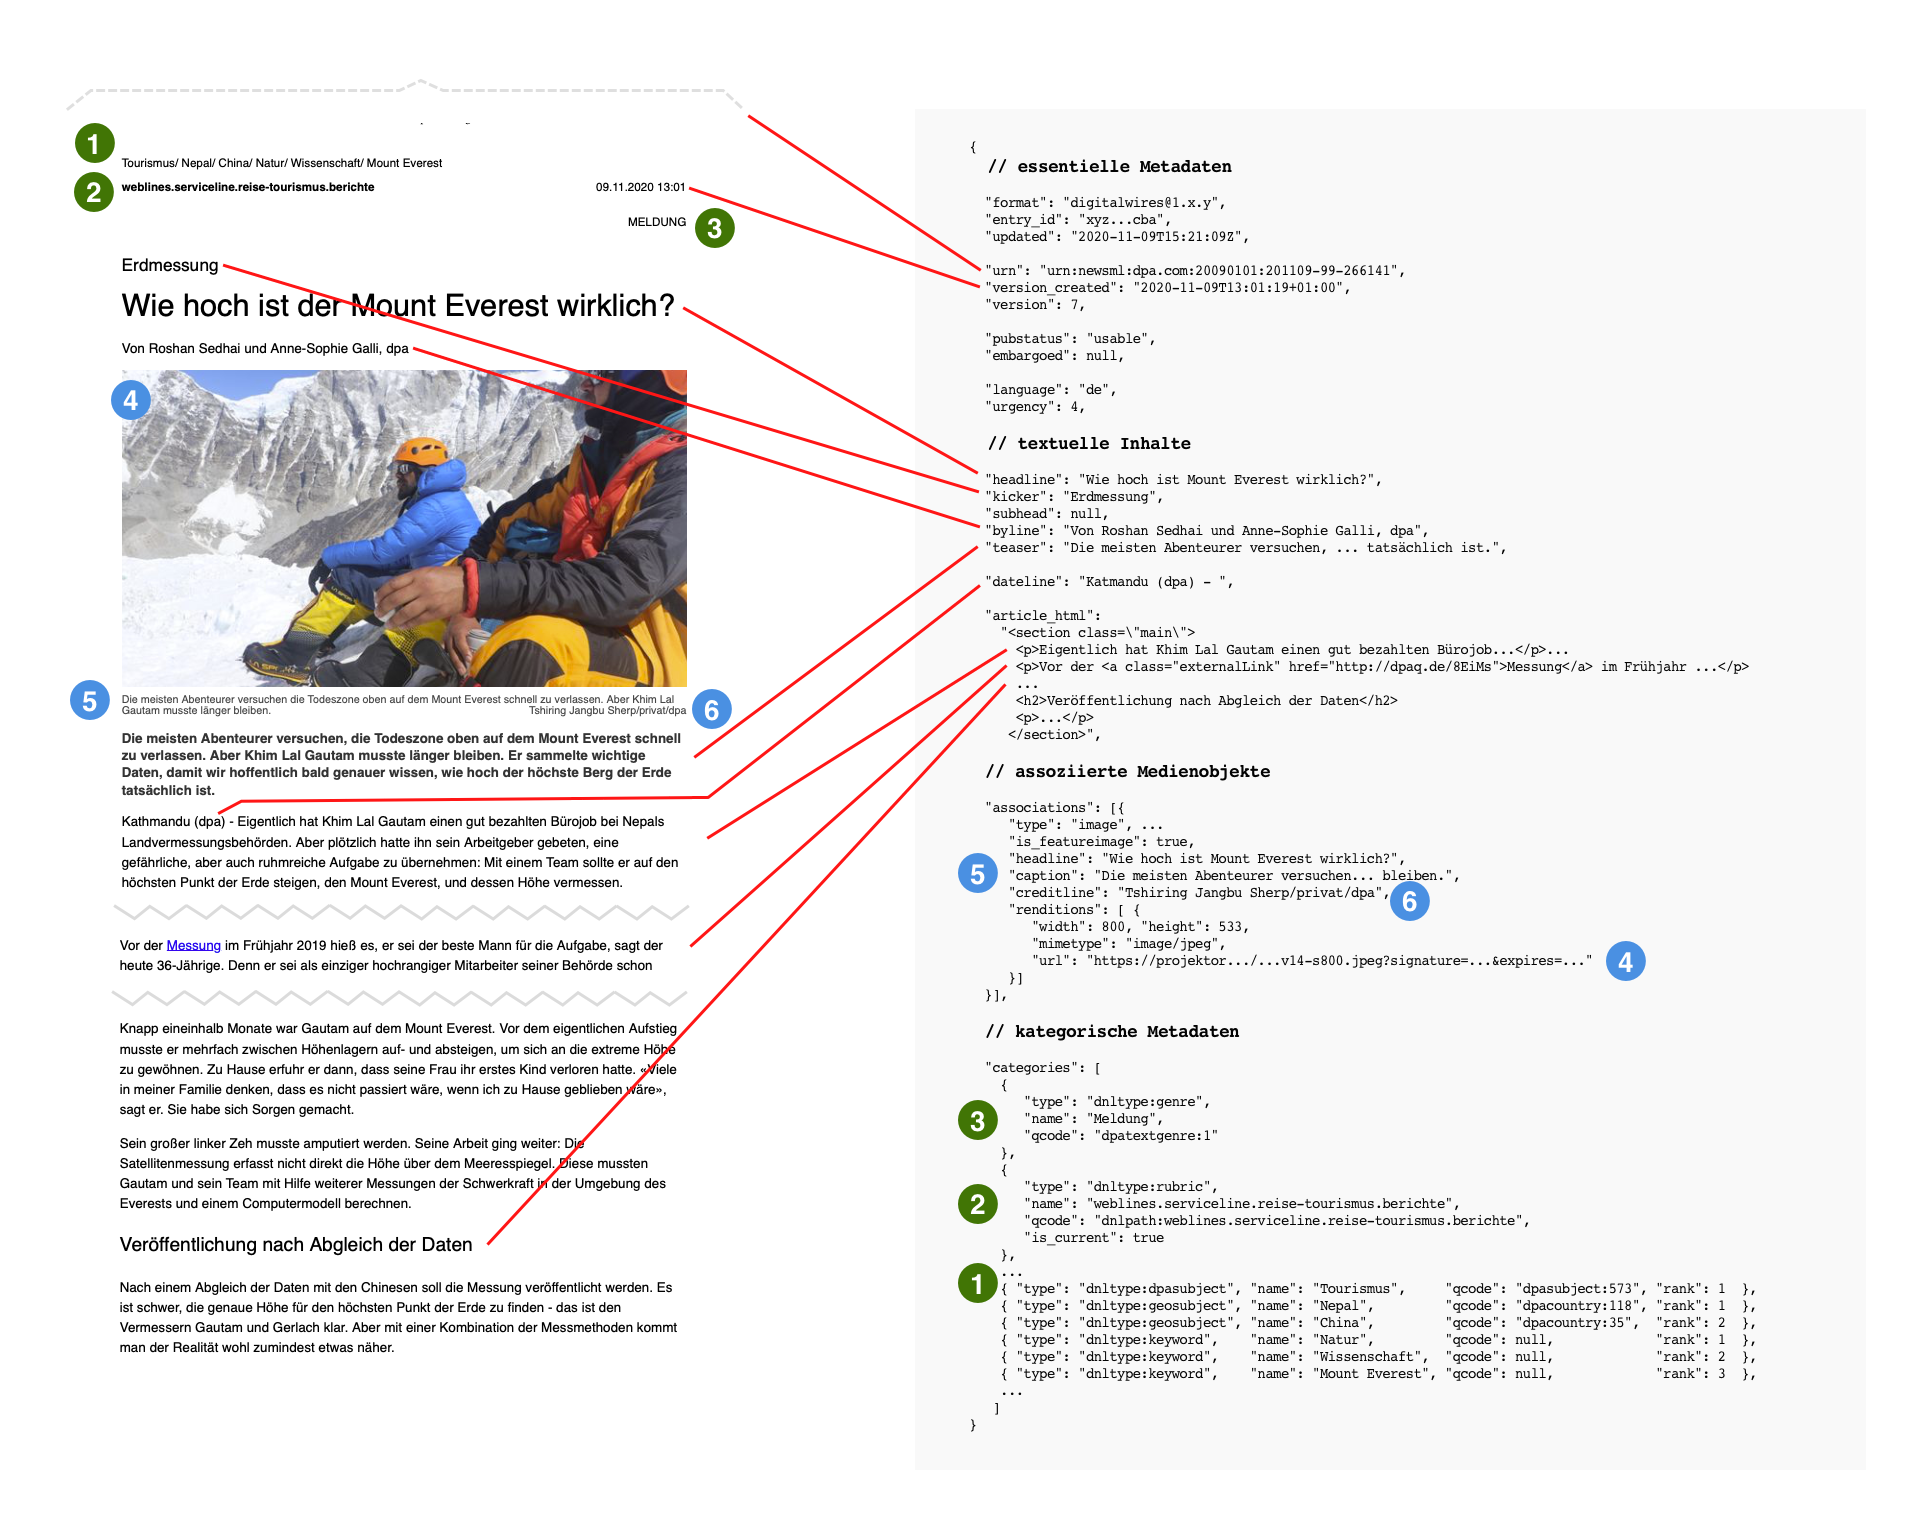
\includegraphics[width=1\linewidth]{abbildungen/dpa doc structure.png}
    \caption{Format dpa Schnittstelle}
    \label{fig:Format dpa Schnittstelle}
    Quelle: \fullcite{DpaApiDocumentation.APIs.2024}
\end{figure}
Als zweite Datenquelle wird die Deutsche Presse Agentur (dpa) angebunden. 
Diese stellt ebenfalls eine API zum konsumieren der Nachrichten bereit, jedoch ist das Angebot wesentlich weitreichender. Grundsätzlich werden drei Formen von Schnittstellen bereitgestellt:

\textbf{s3push-API}
Stellt die Daten im JSON Format über eine event-basierte Kommunikation bereit. Die Implementierung sieht eine direkte Anbindung eines S3 Buckets auf der Seite des Konsumenten vor und ermöglicht so das transportieren von neuen oder aktualisierten Topicles. Durch diesen Ansatz ist die Kommunikation zu der Schnittstelle wenig komplex und effizient, da als Konsument keine Logik zum aktualisieren der Bestandsdaten notwendig ist.\footcite[Vgl.][]{DpaApiDocumentation.APIs.2024}

\textbf{wireQ-API}
Stellt die Daten ebenfalls im JSON Format bereit, jedoch ausgegeben in einer cloud-basierten Warteschlange. Dadurch ist die Implementierung nicht an einem S3 Bucket gebunden, wodurch eine individuelle Kommunikationslogik auf Konsumentenseite notwendig ist. Erhalten bleibt dabei auch der Vorteil der Effizienz, da nur neue oder aktualisierte Daten transportiert werden.\footcite[Vgl.][]{DpaApiDocumentation.APIs.2024}

\textbf{jsonfeed-API}
Stellt die Daten ebenfalls im JSON Format technisch dar, welches strukturell jedoch Atom-XML bzw. RSS Feeds ähnelt. Beim Anfragen der Daten wird ein Vollbezug der verfügbaren Daten gestartet, welcher auch bereits abgefragte Nachrichten enthält. Entsprechend muss auf Konsumentenseite eine entsprechende Geschäftslogik implementiert werden. \footcite[Vgl.][]{DpaApiDocumentation.APIs.2024}

Für den Aufbau einer ersten Iteration der Datensammlungsumgebung ist die Anbindung an die \textit{jsonfeed-API} sinnvoll, da die Anbindung alleinstehend zunächst wenig Komplexität aufweist. 



\newpage
\subsection{Architektur und Design der Datensammlungsumgebung}

Um das Limit der Tagesschau API von 40 Anfragen pro Stunde nicht zu überschreiten, wurde folgender Batch Job konzipiert. 

\begin{figure}
    \centering
    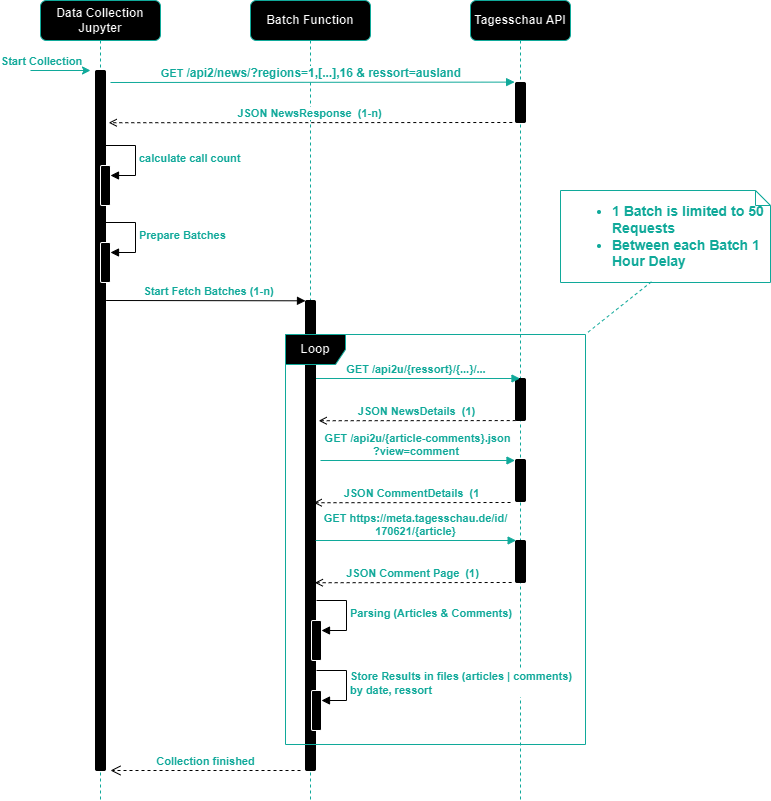
\includegraphics[width=1\linewidth]{abbildungen/image.png}
    \caption{Sequenzdiagramm Abfrage von Tagesschau Daten}
    \label{fig:Sequenzdiagramm Abfrage von Tagesschau Daten}
\end{figure}